\chapter{Divide and Conquer}

\textit{Veni, vidi, vici.} 
\begin{flushright}
    --- Gaius Julius Caesar
\end{flushright}

\section{Introduction}

\term{Divide and Conquer} is a general algorithm design paradigm

\begin{listu}
    \item \textbf{Divide} the problem into smaller subproblems
    \item \textbf{Conquer} the subproblems recursively
    \item \textbf{Combine} the solutions to the subproblems into a solution to the original problem
\end{listu}

\begin{example}[Merge Sort]
    \textsc{MergeSort} is a sorting algorithm that uses the divide and conquer paradigm.

    \begin{listu}
        \item \textbf{Divide}: Split the array into two halves
        \item \textbf{Conquer}: Sort the two halves recursively
        \item \textbf{Combine}: Merge the two sorted halves into a sorted array
    \end{listu}
\end{example}

\begin{remark}
    When analyzing divide and conquer algorithms, \bred{constants} matter due to the recursive nature of the algorithm.
\end{remark}

\subsection{Merge Sort}

Merge sort is a sorting algorithm that uses the divide and conquer paradigm. It divides the array into two halves, sorts the two halves recursively, and merges the two sorted halves into a sorted array.

\begin{algorithm}
    \caption{Merge Sort}

    \begin{algorithmic}[1]
        \Function{MergeSort}{$A$}
            \If{$|A| \le 2$}
                \State \Return \Call{BruteForceSort}{$A$}
            \EndIf
            \State $m \gets \lfloor |A| / 2 \rfloor$
            \State $L \gets \Call{MergeSort}{A[1 \dots m]}$
            \State $R \gets \Call{MergeSort}{A[m+1 \dots |A|]}$
            \State \Return $\Call{Merge}{L, R}$
        \EndFunction
    \end{algorithmic}
\end{algorithm}

\begin{claim}
    Two arrays of length $m$ that are sorted can be combined into a sorted string in $\mathcal{O}(m)$ time.
\end{claim}

\begin{algorithm}
    \caption{Merge}

    \begin{algorithmic}[1]
        \Function{Merge}{$L, R$}
            \State $i \gets 1$
            \State $j \gets 1$
            \State $A \gets \emptyset$
            \While{$i \le |L|$ and $j \le |R|$}
                \If{$L[i] \le R[j]$}
                    \State $A \gets A \cup \{L[i]\}$
                    \State $i \gets i + 1$
                \Else
                    \State $A \gets A \cup \{R[j]\}$
                    \State $j \gets j + 1$
                \EndIf
            \EndWhile
            \State \Return $A \cup L[i \dots] \cup R[j \dots]$
        \EndFunction
    \end{algorithmic}
\end{algorithm}

\begin{center}
    \begin{tikzpicture}
        \node (root) at (0, 0) {$n$};
        \node (l) at (-2, -1)  {$\displaystyle \frac{n}{2^1}$};
        \node (r) at (2, -1)   {$\displaystyle \frac{n}{2^1}$};
        \node (ll) at (-3, -2) {$\displaystyle \frac{n}{2^2}$};
        \node (lr) at (-1, -2) {$\displaystyle \frac{n}{2^2}$};
        \node (rl) at (1, -2)  {$\displaystyle \frac{n}{2^2}$};
        \node (rr) at (3, -2)  {$\displaystyle \frac{n}{2^2}$};
        % dots below the leaves
        \node (llDots) at (-3, -3) {$\vdots$};
        \node (lrDots) at (-1, -3) {$\vdots$};
        \node (rlDots) at (1, -3) {$\vdots$};
        \node (rrDots) at (3, -3) {$\vdots$};


        \draw (root) -- (l);
        \draw (root) -- (r);
        \draw (l) -- (ll);
        \draw (l) -- (lr);
        \draw (r) -- (rl);
        \draw (r) -- (rr);
    \end{tikzpicture}
\end{center}

To compute the cost of \textsc{MergeSort}, we need to compute the cost of \textsc{Merge} and the cost of the levels. 

\begin{claim}
    The cost of the levels is \[
        \left( \frac{n}{2} \right) \cdot \mathcal{O}(2^2) = \mathcal{O}(n)
    \]
\end{claim}

Indeed, in each level $j$, there are $2^j$ subproblems of size $\frac{n}{2^j}$, and the cost of each subproblem is $\mathcal{O}(2^j)$. Thus, the cost of each level is \[
    \left( \frac{n}{2^j} \right) \cdot \mathcal{O}(2^j) = \mathcal{O}(n).
\]

Then, the cost of \textsc{MergeSort} is \[
    \sum_{j=1}^{\log_2 n - 1} \left( \frac{n}{2^j} \right) \cdot \mathcal{O}(2^j) = \mathcal{O}(n \log n)
\]

\begin{claim}
    \textsc{MergeSort} is correct.
\end{claim}

\begin{proof}
    Proof by contradiction. 

    Assume that \textsc{MergeSort} is not correct. 

    % TODO
    TODO: prove on a case by case basis
\end{proof}

\begin{proof}
    Proof by induction on the number of iterations of \textsc{MergeSort}.

    \begin{listu}
        \item \textbf{Base case}: $s(2)$
        
        \textsc{BruteForceSort} is correct by construction.

        \item \textbf{Induction Steps}
        
        Assume \textsc{MergeSort} is correct for any array $s$ of length $L \ge 2$. 

        Without loss of generality, assume $L$ is a power of 2. For the other cases, some extra work is needed.
        
        \begin{center}
            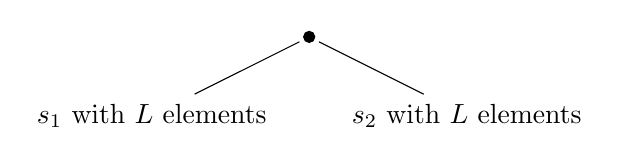
\begin{tikzpicture}
                \node (root) at (0, 0) {};
                \filldraw (root) circle (2pt);
                \node (l) at (-2, -1)  {$s_1$ with $L$ elements};
                \node (r) at (2, -1)   {$s_2$ with $L$ elements};

                \draw (root) -- (l);
                \draw (root) -- (r);
            \end{tikzpicture}
        \end{center}

        If \textsc{MergeSort} is correct, then $s_1$ and $s_2$ are sorted.

        For $j = 1$ to $L$, compare $s_1[j]$ to $s_2[j]$ and insert if $s_1[j] \ge s_2[j]$.

        The algorithm guarantees that inserted $s_1[j] \ge s_2[j]$. Thus, insertion is correct.

        This implies that, in cases of mistake, then the order must have been wrong to start with. 

        This is a contradiction, as we assumed that \textsc{MergeSort} is correct for $L$ elements.

        Thus, \textsc{MergeSort} is correct. 
    \end{listu}
\end{proof}

\subsection{Counting Inversions}

\begin{listu}
    \item \textbf{Problem}
    
    Given an array $a$ of length $n$, count the number of pairs $(i, j)$ such that $i < j$ but $a[i] > a[j]$.

    \item \textbf{Applications}
    
    \begin{listu}
        \item Voting theory
        \item Collaborative filtering 
        \item Measuring the ``sortedness'' of an array
        \item Seneitivity analysis of Google's ranking function 
        \item \dots
    \end{listu}
\end{listu}

\begin{definition}[Inversion]
    An \term{inversion} is a pair $(i, j)$ such that $i < j$ but $a[i] > a[j]$.
\end{definition}

The brute force algorithm is to check all pairs $(i, j)$ and count the number of inversions. This is $\mathcal{O}(n^2)$. We can do better by using the divide and conquer paradigm.

\begin{listu}
    \item \textbf{Divide}: Split the array into two equal halves $x$ and $y$
    \item \textbf{Conquer}: Count the number of inversions in the two halves recursively
    \item \textbf{Combine}:
    \begin{listu}
        \item Count the number of inversions where $i \in x$ and $j \in y$
        \item Add the three counts together
    \end{listu}
\end{listu}

\begin{algorithm}
    \caption{Sort and Count}

    \begin{algorithmic}[1]
        \Function{SortAndCount}{$A$}
            \If{$|A| \le 1$}
                \State \Return $(A, 0)$
            \EndIf
            \State $m \gets \lfloor |A| / 2 \rfloor$
            \State $(L, r_L) \gets \Call{SortAndCount}{A[1 \dots m]}$
            \State $(R, r_R) \gets \Call{SortAndCount}{A[m+1 \dots |A|]}$
            \State $(A', r_{LR}) \gets \Call{MergeAndCount}{L, R}$
            \State \Return $(A', r_L + r_R + r_{LR})$
        \EndFunction
    \end{algorithmic}
\end{algorithm}

Counting inversions $i \in x$ and $j \in y$ is done by merging the two sorted halves.

\begin{listu}
    \item Scan $x$ and $y$ in parallel from left to right
    \item If $x[i] \le y[j]$, then $x[i]$ is not an inversion
    If $x[i] > y[j]$, then $x[i]$ is an inversion with all elements in $y$ that have not been scanned yet
    \item Append the smaller element to the output array
\end{listu}

\newpage
\begin{algorithm}
    \caption{Merge and Count}

    \begin{algorithmic}[1]
        \Function{MergeAndCount}{$L, R$}
            \State $i \gets 1$
            \State $j \gets 1$
            \State $A \gets \emptyset$
            \State $r_{LR} \gets 0$
            \While{$i \le |L|$ and $j \le |R|$}
                \If{$L[i] \le R[j]$}
                    \State $A \gets A \cup \{L[i]\}$
                    \State $i \gets i + 1$
                \Else
                    \State $A \gets A \cup \{R[j]\}$
                    \State $j \gets j + 1$
                    \State $r_{LR} \gets r_{LR} + |L| - i + 1$
                \EndIf
            \EndWhile
            \State \Return $(A \cup L[i \dots] \cup R[j \dots], r_{LR})$
        \EndFunction
    \end{algorithmic}
\end{algorithm}

To formally prove correctness of \textsc{SortAndCount}, we can induce on the size of the array, $n$. 

To analyze the running time of \textsc{SortAndCount}, 

\begin{listu}
    \item Suppose $T(n)$ is the worst-case running time for inputs of size $n$
    \item Our algorithm satisfies $T(n) \le 2T(\frac{n}{2}) + \mathcal{O}(n)$
    \item Master theorem says this is $T(n) = \mathcal{O}(n \log n)$
\end{listu}

\section{Master Theorem}

\begin{theorem}[Master Theorem]\index{Master Theorem}
    Let $a \ge 1$ and $b > 1$ be constants, let $f(n)$ be a function, and let $T(n)$ be defined on the nonnegative integers by the recurrence \[
        T(n) \le a \cdot T\left( \frac{n}{b} \right) + f(n)
    \]

    where we interpret $n/b$ to mean either $\lfloor n/b \rfloor$ or $\lceil n/b \rceil$. 
    
    Let $d = \log_b a$. Then, $T(n)$ has the following asymptotic bounds:
    \begin{enumerate}
        \item If $f(n) = \mathcal{O}(n^{d - \epsilon})$ for some constant $\epsilon > 0$, then $T(n) = \mathcal{O}(n^d)$.

        This is the \bred{merge heavy} case. The cost of merging dominates the cost of recursion.

        \item If $f(n) = \mathcal{O}(n^d \log^k n)$, then $T(n) = \mathcal{O}(n^d \log^{k+1} n)$.

        This is the \bred{balanced} case. The cost of merging and recursion are the same.

        \item If $f(n) = \mathcal{O}(n^{d + \epsilon})$ for some constant $\epsilon > 0$, then $T(n) = \mathcal{O}(f(n))$.

        This is the \bred{leaf (recursion) heavy} case. The cost of recursion dominates the cost of merging.
    \end{enumerate}
\end{theorem}

\subsection{Closest Pair}

\begin{listu}
    \item \textbf{Problem}
    
    Given $n$ points of the form $(x_i, y_i)$ in the plane, find the closest pair of points.

    \item \textbf{Applications}
    
    \begin{listu}
        \item Basic primitive in graphics and computer vision
        \item Geographic information systems, molecular modeling, air traffic control
        \item Special case of nearest neighbor
    \end{listu}

    \item \textbf{Brute force} is $\mathcal{O}(n^2)$.
\end{listu}

We can use the divide and conquer paradigm to solve this problem.

\begin{listu}
    \item \textbf{Divide}: Split the points into two equal halves by drawing a vertical line $L$ through the median $x$-coordinate

    \begin{center} \includegraphics[width=0.5\linewidth]{figures/Closest Pair Divide.png} \end{center}

    \item \textbf{Conquer}: Find the closest pair of points in each half recursively

    \item \textbf{Combine}: Find the closest pair of points with one point in each half

    We can restrict our attention to points within $\delta$ of $L$ on each side, where $\delta = $ best of the solutions within the two halves. 

    \begin{center} \includegraphics[width=0.5\linewidth]{figures/Closest Pair Conquer.png} \end{center}

    \begin{listu}
        \item Only need to look at points within $\delta$ of $L$ on each side
        \item Sort points on the strip by $y$ coordinate
        \item Only need to check each point with next 11 points in sorted list
    \end{listu}

    \begin{remark}
        \begin{minipage}[t]{0.55\linewidth}
            We chose the number $11$ on purpose.

            \begin{claim}
                If two points are at least $12$ positions apart in the sorted list, their distance is at least $\delta$. 
            \end{claim}

            \begin{proof}
                {~~~}

                \begin{listu}
                    \item No two points lie in the same $\frac{\delta}{2} \times \delta$ rectangle. 
                    
                    \item Two points that are more than two rows apart are at distance $\delta$. 
                \end{listu}
            \end{proof}
        \end{minipage}
        \hfill
        \begin{minipage}[t]{0.4\linewidth}
            \begin{center} \raisebox{-0.9\height}{ \includegraphics[width=0.9\linewidth]{figures/Closest Pair Grid.png} } \end{center}
        \end{minipage}
    \end{remark}

    \item Return the best of 3 solutions
\end{listu}

Let $T(n)$ be the worst-case running time of the algorithm. To analyze the Running time for the combine operation, 
\begin{listu}
    \item Finding points on the strip is $\mathcal{O}(n)$
    \item Sorting points on the strip by their $y$-coordinate is $\mathcal{O}(n \log n)$
    \item Testing each point against 11 points is $\mathcal{O}(n)$
\end{listu}

Thus, the total running running time is \[
    T(n) \le 2T\left( \frac{n}{2} \right) + \mathcal{O}(n \log n)
\] 

By the master theorem, this yields $T(n) = \mathcal{O}(n \log n)$.